% Options for packages loaded elsewhere
\PassOptionsToPackage{unicode}{hyperref}
\PassOptionsToPackage{hyphens}{url}
\PassOptionsToPackage{dvipsnames,svgnames,x11names}{xcolor}
%
\documentclass[
  letterpaper,
  DIV=11,
  numbers=noendperiod]{scrartcl}

\usepackage{amsmath,amssymb}
\usepackage{iftex}
\ifPDFTeX
  \usepackage[T1]{fontenc}
  \usepackage[utf8]{inputenc}
  \usepackage{textcomp} % provide euro and other symbols
\else % if luatex or xetex
  \usepackage{unicode-math}
  \defaultfontfeatures{Scale=MatchLowercase}
  \defaultfontfeatures[\rmfamily]{Ligatures=TeX,Scale=1}
\fi
\usepackage{lmodern}
\ifPDFTeX\else  
    % xetex/luatex font selection
\fi
% Use upquote if available, for straight quotes in verbatim environments
\IfFileExists{upquote.sty}{\usepackage{upquote}}{}
\IfFileExists{microtype.sty}{% use microtype if available
  \usepackage[]{microtype}
  \UseMicrotypeSet[protrusion]{basicmath} % disable protrusion for tt fonts
}{}
\makeatletter
\@ifundefined{KOMAClassName}{% if non-KOMA class
  \IfFileExists{parskip.sty}{%
    \usepackage{parskip}
  }{% else
    \setlength{\parindent}{0pt}
    \setlength{\parskip}{6pt plus 2pt minus 1pt}}
}{% if KOMA class
  \KOMAoptions{parskip=half}}
\makeatother
\usepackage{xcolor}
\setlength{\emergencystretch}{3em} % prevent overfull lines
\setcounter{secnumdepth}{-\maxdimen} % remove section numbering
% Make \paragraph and \subparagraph free-standing
\makeatletter
\ifx\paragraph\undefined\else
  \let\oldparagraph\paragraph
  \renewcommand{\paragraph}{
    \@ifstar
      \xxxParagraphStar
      \xxxParagraphNoStar
  }
  \newcommand{\xxxParagraphStar}[1]{\oldparagraph*{#1}\mbox{}}
  \newcommand{\xxxParagraphNoStar}[1]{\oldparagraph{#1}\mbox{}}
\fi
\ifx\subparagraph\undefined\else
  \let\oldsubparagraph\subparagraph
  \renewcommand{\subparagraph}{
    \@ifstar
      \xxxSubParagraphStar
      \xxxSubParagraphNoStar
  }
  \newcommand{\xxxSubParagraphStar}[1]{\oldsubparagraph*{#1}\mbox{}}
  \newcommand{\xxxSubParagraphNoStar}[1]{\oldsubparagraph{#1}\mbox{}}
\fi
\makeatother

\usepackage{color}
\usepackage{fancyvrb}
\newcommand{\VerbBar}{|}
\newcommand{\VERB}{\Verb[commandchars=\\\{\}]}
\DefineVerbatimEnvironment{Highlighting}{Verbatim}{commandchars=\\\{\}}
% Add ',fontsize=\small' for more characters per line
\usepackage{framed}
\definecolor{shadecolor}{RGB}{241,243,245}
\newenvironment{Shaded}{\begin{snugshade}}{\end{snugshade}}
\newcommand{\AlertTok}[1]{\textcolor[rgb]{0.68,0.00,0.00}{#1}}
\newcommand{\AnnotationTok}[1]{\textcolor[rgb]{0.37,0.37,0.37}{#1}}
\newcommand{\AttributeTok}[1]{\textcolor[rgb]{0.40,0.45,0.13}{#1}}
\newcommand{\BaseNTok}[1]{\textcolor[rgb]{0.68,0.00,0.00}{#1}}
\newcommand{\BuiltInTok}[1]{\textcolor[rgb]{0.00,0.23,0.31}{#1}}
\newcommand{\CharTok}[1]{\textcolor[rgb]{0.13,0.47,0.30}{#1}}
\newcommand{\CommentTok}[1]{\textcolor[rgb]{0.37,0.37,0.37}{#1}}
\newcommand{\CommentVarTok}[1]{\textcolor[rgb]{0.37,0.37,0.37}{\textit{#1}}}
\newcommand{\ConstantTok}[1]{\textcolor[rgb]{0.56,0.35,0.01}{#1}}
\newcommand{\ControlFlowTok}[1]{\textcolor[rgb]{0.00,0.23,0.31}{\textbf{#1}}}
\newcommand{\DataTypeTok}[1]{\textcolor[rgb]{0.68,0.00,0.00}{#1}}
\newcommand{\DecValTok}[1]{\textcolor[rgb]{0.68,0.00,0.00}{#1}}
\newcommand{\DocumentationTok}[1]{\textcolor[rgb]{0.37,0.37,0.37}{\textit{#1}}}
\newcommand{\ErrorTok}[1]{\textcolor[rgb]{0.68,0.00,0.00}{#1}}
\newcommand{\ExtensionTok}[1]{\textcolor[rgb]{0.00,0.23,0.31}{#1}}
\newcommand{\FloatTok}[1]{\textcolor[rgb]{0.68,0.00,0.00}{#1}}
\newcommand{\FunctionTok}[1]{\textcolor[rgb]{0.28,0.35,0.67}{#1}}
\newcommand{\ImportTok}[1]{\textcolor[rgb]{0.00,0.46,0.62}{#1}}
\newcommand{\InformationTok}[1]{\textcolor[rgb]{0.37,0.37,0.37}{#1}}
\newcommand{\KeywordTok}[1]{\textcolor[rgb]{0.00,0.23,0.31}{\textbf{#1}}}
\newcommand{\NormalTok}[1]{\textcolor[rgb]{0.00,0.23,0.31}{#1}}
\newcommand{\OperatorTok}[1]{\textcolor[rgb]{0.37,0.37,0.37}{#1}}
\newcommand{\OtherTok}[1]{\textcolor[rgb]{0.00,0.23,0.31}{#1}}
\newcommand{\PreprocessorTok}[1]{\textcolor[rgb]{0.68,0.00,0.00}{#1}}
\newcommand{\RegionMarkerTok}[1]{\textcolor[rgb]{0.00,0.23,0.31}{#1}}
\newcommand{\SpecialCharTok}[1]{\textcolor[rgb]{0.37,0.37,0.37}{#1}}
\newcommand{\SpecialStringTok}[1]{\textcolor[rgb]{0.13,0.47,0.30}{#1}}
\newcommand{\StringTok}[1]{\textcolor[rgb]{0.13,0.47,0.30}{#1}}
\newcommand{\VariableTok}[1]{\textcolor[rgb]{0.07,0.07,0.07}{#1}}
\newcommand{\VerbatimStringTok}[1]{\textcolor[rgb]{0.13,0.47,0.30}{#1}}
\newcommand{\WarningTok}[1]{\textcolor[rgb]{0.37,0.37,0.37}{\textit{#1}}}

\providecommand{\tightlist}{%
  \setlength{\itemsep}{0pt}\setlength{\parskip}{0pt}}\usepackage{longtable,booktabs,array}
\usepackage{calc} % for calculating minipage widths
% Correct order of tables after \paragraph or \subparagraph
\usepackage{etoolbox}
\makeatletter
\patchcmd\longtable{\par}{\if@noskipsec\mbox{}\fi\par}{}{}
\makeatother
% Allow footnotes in longtable head/foot
\IfFileExists{footnotehyper.sty}{\usepackage{footnotehyper}}{\usepackage{footnote}}
\makesavenoteenv{longtable}
\usepackage{graphicx}
\makeatletter
\newsavebox\pandoc@box
\newcommand*\pandocbounded[1]{% scales image to fit in text height/width
  \sbox\pandoc@box{#1}%
  \Gscale@div\@tempa{\textheight}{\dimexpr\ht\pandoc@box+\dp\pandoc@box\relax}%
  \Gscale@div\@tempb{\linewidth}{\wd\pandoc@box}%
  \ifdim\@tempb\p@<\@tempa\p@\let\@tempa\@tempb\fi% select the smaller of both
  \ifdim\@tempa\p@<\p@\scalebox{\@tempa}{\usebox\pandoc@box}%
  \else\usebox{\pandoc@box}%
  \fi%
}
% Set default figure placement to htbp
\def\fps@figure{htbp}
\makeatother

\KOMAoption{captions}{tableheading}
\makeatletter
\@ifpackageloaded{caption}{}{\usepackage{caption}}
\AtBeginDocument{%
\ifdefined\contentsname
  \renewcommand*\contentsname{Table of contents}
\else
  \newcommand\contentsname{Table of contents}
\fi
\ifdefined\listfigurename
  \renewcommand*\listfigurename{List of Figures}
\else
  \newcommand\listfigurename{List of Figures}
\fi
\ifdefined\listtablename
  \renewcommand*\listtablename{List of Tables}
\else
  \newcommand\listtablename{List of Tables}
\fi
\ifdefined\figurename
  \renewcommand*\figurename{Figure}
\else
  \newcommand\figurename{Figure}
\fi
\ifdefined\tablename
  \renewcommand*\tablename{Table}
\else
  \newcommand\tablename{Table}
\fi
}
\@ifpackageloaded{float}{}{\usepackage{float}}
\floatstyle{ruled}
\@ifundefined{c@chapter}{\newfloat{codelisting}{h}{lop}}{\newfloat{codelisting}{h}{lop}[chapter]}
\floatname{codelisting}{Listing}
\newcommand*\listoflistings{\listof{codelisting}{List of Listings}}
\makeatother
\makeatletter
\makeatother
\makeatletter
\@ifpackageloaded{caption}{}{\usepackage{caption}}
\@ifpackageloaded{subcaption}{}{\usepackage{subcaption}}
\makeatother

\usepackage{bookmark}

\IfFileExists{xurl.sty}{\usepackage{xurl}}{} % add URL line breaks if available
\urlstyle{same} % disable monospaced font for URLs
\hypersetup{
  pdftitle={Multinomial Logit Model},
  pdfauthor={Vidhi Vashishth},
  colorlinks=true,
  linkcolor={blue},
  filecolor={Maroon},
  citecolor={Blue},
  urlcolor={Blue},
  pdfcreator={LaTeX via pandoc}}


\title{Multinomial Logit Model}
\author{Vidhi Vashishth}
\date{2025-05-17}

\begin{document}
\maketitle


This assignment explores two methods for estimating the MNL model: (1)
via Maximum Likelihood, and (2) via a Bayesian approach using a
Metropolis-Hastings MCMC algorithm.

\subsection{1. Likelihood for the Multi-nomial Logit (MNL)
Model}\label{likelihood-for-the-multi-nomial-logit-mnl-model}

Suppose we have \(i=1,\ldots,n\) consumers who each select exactly one
product \(j\) from a set of \(J\) products. The outcome variable is the
identity of the product chosen \(y_i \in \{1, \ldots, J\}\) or
equivalently a vector of \(J-1\) zeros and \(1\) one, where the \(1\)
indicates the selected product. For example, if the third product was
chosen out of 3 products, then either \(y=3\) or \(y=(0,0,1)\) depending
on how we want to represent it. Suppose also that we have a vector of
data on each product \(x_j\) (eg, brand, price, etc.).

We model the consumer's decision as the selection of the product that
provides the most utility, and we'll specify the utility function as a
linear function of the product characteristics:

\[ U_{ij} = x_j'\beta + \epsilon_{ij} \]

where \(\epsilon_{ij}\) is an i.i.d. extreme value error term.

The choice of the i.i.d. extreme value error term leads to a closed-form
expression for the probability that consumer \(i\) chooses product
\(j\):

\[ \mathbb{P}_i(j) = \frac{e^{x_j'\beta}}{\sum_{k=1}^Je^{x_k'\beta}} \]

For example, if there are 3 products, the probability that consumer
\(i\) chooses product 3 is:

\[ \mathbb{P}_i(3) = \frac{e^{x_3'\beta}}{e^{x_1'\beta} + e^{x_2'\beta} + e^{x_3'\beta}} \]

A clever way to write the individual likelihood function for consumer
\(i\) is the product of the \(J\) probabilities, each raised to the
power of an indicator variable (\(\delta_{ij}\)) that indicates the
chosen product:

\[ L_i(\beta) = \prod_{j=1}^J \mathbb{P}_i(j)^{\delta_{ij}} = \mathbb{P}_i(1)^{\delta_{i1}} \times \ldots \times \mathbb{P}_i(J)^{\delta_{iJ}}\]

Notice that if the consumer selected product \(j=3\), then
\(\delta_{i3}=1\) while \(\delta_{i1}=\delta_{i2}=0\) and the likelihood
is:

\[ L_i(\beta) = \mathbb{P}_i(1)^0 \times \mathbb{P}_i(2)^0 \times \mathbb{P}_i(3)^1 = \mathbb{P}_i(3) = \frac{e^{x_3'\beta}}{\sum_{k=1}^3e^{x_k'\beta}} \]

The joint likelihood (across all consumers) is the product of the \(n\)
individual likelihoods:

\[ L_n(\beta) = \prod_{i=1}^n L_i(\beta) = \prod_{i=1}^n \prod_{j=1}^J \mathbb{P}_i(j)^{\delta_{ij}} \]

And the joint log-likelihood function is:

\[ \ell_n(\beta) = \sum_{i=1}^n \sum_{j=1}^J \delta_{ij} \log(\mathbb{P}_i(j)) \]

\subsection{2. Simulate Conjoint Data}\label{simulate-conjoint-data}

We will simulate data from a conjoint experiment about video content
streaming services. We elect to simulate 100 respondents, each
completing 10 choice tasks, where they choose from three alternatives
per task. For simplicity, there is not a ``no choice'' option; each
simulated respondent must select one of the 3 alternatives.

Each alternative is a hypothetical streaming offer consistent of three
attributes: (1) brand is either Netflix, Amazon Prime, or Hulu; (2) ads
can either be part of the experience, or it can be ad-free, and (3)
price per month ranges from \$4 to \$32 in increments of \$4.

The part-worths (ie, preference weights or beta parameters) for the
attribute levels will be 1.0 for Netflix, 0.5 for Amazon Prime (with 0
for Hulu as the reference brand); -0.8 for included adverstisements (0
for ad-free); and -0.1*price so that utility to consumer \(i\) for
hypothethical streaming service \(j\) is

\[
u_{ij} = (1 \times Netflix_j) + (0.5 \times Prime_j) + (-0.8*Ads_j) - 0.1\times Price_j + \varepsilon_{ij}
\]

where the variables are binary indicators and \(\varepsilon\) is Type 1
Extreme Value (ie, Gumble) distributed.

The following code provides the simulation of the conjoint data.

\begin{Shaded}
\begin{Highlighting}[]
\CommentTok{\# Install TinyTeX from R}
\FunctionTok{install.packages}\NormalTok{(}\StringTok{"tinytex"}\NormalTok{)}
\end{Highlighting}
\end{Shaded}

\begin{verbatim}
Updating HTML index of packages in '.Library'
\end{verbatim}

\begin{verbatim}
Making 'packages.html' ... done
\end{verbatim}

\begin{Shaded}
\begin{Highlighting}[]
\NormalTok{tinytex}\SpecialCharTok{::}\FunctionTok{install\_tinytex}\NormalTok{(}\AttributeTok{force =} \ConstantTok{TRUE}\NormalTok{)}
\end{Highlighting}
\end{Shaded}

\begin{verbatim}
tlmgr option sys_bin ~/bin
tlmgr option repository 'https://us.mirrors.cicku.me/ctan/systems/texlive/tlnet'
tlmgr update --list
\end{verbatim}

\begin{Shaded}
\begin{Highlighting}[]
\CommentTok{\# Then specifically install the lmodern package}
\NormalTok{tinytex}\SpecialCharTok{::}\FunctionTok{tlmgr\_install}\NormalTok{(}\StringTok{"lmodern"}\NormalTok{)}
\end{Highlighting}
\end{Shaded}

\begin{verbatim}
tlmgr install lmodern
tlmgr update --self
tlmgr install lmodern
\end{verbatim}

\begin{Shaded}
\begin{Highlighting}[]
\CommentTok{\# set seed for reproducibility}
\FunctionTok{set.seed}\NormalTok{(}\DecValTok{123}\NormalTok{)}

\CommentTok{\# define attributes}
\NormalTok{brand }\OtherTok{\textless{}{-}} \FunctionTok{c}\NormalTok{(}\StringTok{"N"}\NormalTok{, }\StringTok{"P"}\NormalTok{, }\StringTok{"H"}\NormalTok{) }\CommentTok{\# Netflix, Prime, Hulu}
\NormalTok{ad }\OtherTok{\textless{}{-}} \FunctionTok{c}\NormalTok{(}\StringTok{"Yes"}\NormalTok{, }\StringTok{"No"}\NormalTok{)}
\NormalTok{price }\OtherTok{\textless{}{-}} \FunctionTok{seq}\NormalTok{(}\DecValTok{8}\NormalTok{, }\DecValTok{32}\NormalTok{, }\AttributeTok{by=}\DecValTok{4}\NormalTok{)}

\CommentTok{\# generate all possible profiles}
\NormalTok{profiles }\OtherTok{\textless{}{-}} \FunctionTok{expand.grid}\NormalTok{(}
    \AttributeTok{brand =}\NormalTok{ brand,}
    \AttributeTok{ad =}\NormalTok{ ad,}
    \AttributeTok{price =}\NormalTok{ price}
\NormalTok{)}
\NormalTok{m }\OtherTok{\textless{}{-}} \FunctionTok{nrow}\NormalTok{(profiles)}

\CommentTok{\# assign part{-}worth utilities (true parameters)}
\NormalTok{b\_util }\OtherTok{\textless{}{-}} \FunctionTok{c}\NormalTok{(}\AttributeTok{N =} \FloatTok{1.0}\NormalTok{, }\AttributeTok{P =} \FloatTok{0.5}\NormalTok{, }\AttributeTok{H =} \DecValTok{0}\NormalTok{)}
\NormalTok{a\_util }\OtherTok{\textless{}{-}} \FunctionTok{c}\NormalTok{(}\AttributeTok{Yes =} \SpecialCharTok{{-}}\FloatTok{0.8}\NormalTok{, }\AttributeTok{No =} \FloatTok{0.0}\NormalTok{)}
\NormalTok{p\_util }\OtherTok{\textless{}{-}} \ControlFlowTok{function}\NormalTok{(p) }\SpecialCharTok{{-}}\FloatTok{0.1} \SpecialCharTok{*}\NormalTok{ p}

\CommentTok{\# number of respondents, choice tasks, and alternatives per task}
\NormalTok{n\_peeps }\OtherTok{\textless{}{-}} \DecValTok{100}
\NormalTok{n\_tasks }\OtherTok{\textless{}{-}} \DecValTok{10}
\NormalTok{n\_alts }\OtherTok{\textless{}{-}} \DecValTok{3}

\CommentTok{\# function to simulate one respondent’s data}
\NormalTok{sim\_one }\OtherTok{\textless{}{-}} \ControlFlowTok{function}\NormalTok{(id) \{}
  
\NormalTok{    datlist }\OtherTok{\textless{}{-}} \FunctionTok{list}\NormalTok{()}
    
    \CommentTok{\# loop over choice tasks}
    \ControlFlowTok{for}\NormalTok{ (t }\ControlFlowTok{in} \DecValTok{1}\SpecialCharTok{:}\NormalTok{n\_tasks) \{}
        
        \CommentTok{\# randomly sample 3 alts (better practice would be to use a design)}
\NormalTok{        dat }\OtherTok{\textless{}{-}} \FunctionTok{cbind}\NormalTok{(}\AttributeTok{resp=}\NormalTok{id, }\AttributeTok{task=}\NormalTok{t, profiles[}\FunctionTok{sample}\NormalTok{(m, }\AttributeTok{size=}\NormalTok{n\_alts), ])}
        
        \CommentTok{\# compute deterministic portion of utility}
\NormalTok{        dat}\SpecialCharTok{$}\NormalTok{v }\OtherTok{\textless{}{-}}\NormalTok{ b\_util[dat}\SpecialCharTok{$}\NormalTok{brand] }\SpecialCharTok{+}\NormalTok{ a\_util[dat}\SpecialCharTok{$}\NormalTok{ad] }\SpecialCharTok{+} \FunctionTok{p\_util}\NormalTok{(dat}\SpecialCharTok{$}\NormalTok{price) }\SpecialCharTok{|\textgreater{}} \FunctionTok{round}\NormalTok{(}\DecValTok{10}\NormalTok{)}
        
        \CommentTok{\# add Gumbel noise (Type I extreme value)}
\NormalTok{        dat}\SpecialCharTok{$}\NormalTok{e }\OtherTok{\textless{}{-}} \SpecialCharTok{{-}}\FunctionTok{log}\NormalTok{(}\SpecialCharTok{{-}}\FunctionTok{log}\NormalTok{(}\FunctionTok{runif}\NormalTok{(n\_alts)))}
\NormalTok{        dat}\SpecialCharTok{$}\NormalTok{u }\OtherTok{\textless{}{-}}\NormalTok{ dat}\SpecialCharTok{$}\NormalTok{v }\SpecialCharTok{+}\NormalTok{ dat}\SpecialCharTok{$}\NormalTok{e}
        
        \CommentTok{\# identify chosen alternative}
\NormalTok{        dat}\SpecialCharTok{$}\NormalTok{choice }\OtherTok{\textless{}{-}} \FunctionTok{as.integer}\NormalTok{(dat}\SpecialCharTok{$}\NormalTok{u }\SpecialCharTok{==} \FunctionTok{max}\NormalTok{(dat}\SpecialCharTok{$}\NormalTok{u))}
        
        \CommentTok{\# store task}
\NormalTok{        datlist[[t]] }\OtherTok{\textless{}{-}}\NormalTok{ dat}
\NormalTok{    \}}
    
    \CommentTok{\# combine all tasks for one respondent}
    \FunctionTok{do.call}\NormalTok{(rbind, datlist)}
\NormalTok{\}}

\CommentTok{\# simulate data for all respondents}
\NormalTok{conjoint\_data }\OtherTok{\textless{}{-}} \FunctionTok{do.call}\NormalTok{(rbind, }\FunctionTok{lapply}\NormalTok{(}\DecValTok{1}\SpecialCharTok{:}\NormalTok{n\_peeps, sim\_one))}

\CommentTok{\# remove values unobservable to the researcher}
\NormalTok{conjoint\_data }\OtherTok{\textless{}{-}}\NormalTok{ conjoint\_data[ , }\FunctionTok{c}\NormalTok{(}\StringTok{"resp"}\NormalTok{, }\StringTok{"task"}\NormalTok{, }\StringTok{"brand"}\NormalTok{, }\StringTok{"ad"}\NormalTok{, }\StringTok{"price"}\NormalTok{, }\StringTok{"choice"}\NormalTok{)]}

\CommentTok{\# clean up}
\FunctionTok{rm}\NormalTok{(}\AttributeTok{list=}\FunctionTok{setdiff}\NormalTok{(}\FunctionTok{ls}\NormalTok{(), }\StringTok{"conjoint\_data"}\NormalTok{))}
\end{Highlighting}
\end{Shaded}

\subsection{3. Preparing the Data for
Estimation}\label{preparing-the-data-for-estimation}

The ``hard part'' of the MNL likelihood function is organizing the data,
as we need to keep track of 3 dimensions (consumer \(i\), covariate
\(k\), and product \(j\)) instead of the typical 2 dimensions for
cross-sectional regression models (consumer \(i\) and covariate \(k\)).
The fact that each task for each respondent has the same number of
alternatives (3) helps. In addition, we need to convert the categorical
variables for brand and ads into binary variables.

\begin{Shaded}
\begin{Highlighting}[]
\CommentTok{\# Examine the structure of the conjoint data}
\NormalTok{conjoint\_data }\OtherTok{\textless{}{-}} \FunctionTok{read.csv}\NormalTok{(}\StringTok{"conjoint\_data.csv"}\NormalTok{)}
\FunctionTok{head}\NormalTok{(conjoint\_data)}
\end{Highlighting}
\end{Shaded}

\begin{verbatim}
  resp task choice brand  ad price
1    1    1      1     N Yes    28
2    1    1      0     H Yes    16
3    1    1      0     P Yes    16
4    1    2      0     N Yes    32
5    1    2      1     P Yes    16
6    1    2      0     N Yes    24
\end{verbatim}

\begin{Shaded}
\begin{Highlighting}[]
\CommentTok{\# Create dummy variables for brands (using Hulu as reference level)}
\NormalTok{conjoint\_data}\SpecialCharTok{$}\NormalTok{netflix }\OtherTok{\textless{}{-}} \FunctionTok{ifelse}\NormalTok{(conjoint\_data}\SpecialCharTok{$}\NormalTok{brand }\SpecialCharTok{==} \StringTok{"N"}\NormalTok{, }\DecValTok{1}\NormalTok{, }\DecValTok{0}\NormalTok{)}
\NormalTok{conjoint\_data}\SpecialCharTok{$}\NormalTok{prime }\OtherTok{\textless{}{-}} \FunctionTok{ifelse}\NormalTok{(conjoint\_data}\SpecialCharTok{$}\NormalTok{brand }\SpecialCharTok{==} \StringTok{"P"}\NormalTok{, }\DecValTok{1}\NormalTok{, }\DecValTok{0}\NormalTok{)}

\CommentTok{\# Create dummy variable for ads (No ads is reference)}
\NormalTok{conjoint\_data}\SpecialCharTok{$}\NormalTok{ads }\OtherTok{\textless{}{-}} \FunctionTok{ifelse}\NormalTok{(conjoint\_data}\SpecialCharTok{$}\NormalTok{ad }\SpecialCharTok{==} \StringTok{"Yes"}\NormalTok{, }\DecValTok{1}\NormalTok{, }\DecValTok{0}\NormalTok{)}

\CommentTok{\# Organize data in format suitable for MNL estimation}
\CommentTok{\# Number of respondents, tasks, and alternatives per task}
\NormalTok{n\_resp }\OtherTok{\textless{}{-}} \FunctionTok{length}\NormalTok{(}\FunctionTok{unique}\NormalTok{(conjoint\_data}\SpecialCharTok{$}\NormalTok{resp))}
\NormalTok{n\_tasks }\OtherTok{\textless{}{-}} \FunctionTok{length}\NormalTok{(}\FunctionTok{unique}\NormalTok{(conjoint\_data}\SpecialCharTok{$}\NormalTok{task))}
\NormalTok{n\_obs }\OtherTok{\textless{}{-}}\NormalTok{ n\_resp }\SpecialCharTok{*}\NormalTok{ n\_tasks}
\NormalTok{n\_alts }\OtherTok{\textless{}{-}} \DecValTok{3}

\CommentTok{\# Initialize arrays to store the data}
\NormalTok{choices }\OtherTok{\textless{}{-}} \FunctionTok{array}\NormalTok{(}\DecValTok{0}\NormalTok{, }\AttributeTok{dim =} \FunctionTok{c}\NormalTok{(n\_obs, n\_alts))}
\NormalTok{X\_netflix }\OtherTok{\textless{}{-}} \FunctionTok{array}\NormalTok{(}\DecValTok{0}\NormalTok{, }\AttributeTok{dim =} \FunctionTok{c}\NormalTok{(n\_obs, n\_alts))}
\NormalTok{X\_prime }\OtherTok{\textless{}{-}} \FunctionTok{array}\NormalTok{(}\DecValTok{0}\NormalTok{, }\AttributeTok{dim =} \FunctionTok{c}\NormalTok{(n\_obs, n\_alts))}
\NormalTok{X\_ads }\OtherTok{\textless{}{-}} \FunctionTok{array}\NormalTok{(}\DecValTok{0}\NormalTok{, }\AttributeTok{dim =} \FunctionTok{c}\NormalTok{(n\_obs, n\_alts))}
\NormalTok{X\_price }\OtherTok{\textless{}{-}} \FunctionTok{array}\NormalTok{(}\DecValTok{0}\NormalTok{, }\AttributeTok{dim =} \FunctionTok{c}\NormalTok{(n\_obs, n\_alts))}

\CommentTok{\# Populate the arrays}
\NormalTok{row\_idx }\OtherTok{\textless{}{-}} \DecValTok{0}
\ControlFlowTok{for}\NormalTok{ (r }\ControlFlowTok{in} \FunctionTok{unique}\NormalTok{(conjoint\_data}\SpecialCharTok{$}\NormalTok{resp)) \{}
  \ControlFlowTok{for}\NormalTok{ (t }\ControlFlowTok{in} \DecValTok{1}\SpecialCharTok{:}\NormalTok{n\_tasks) \{}
\NormalTok{    row\_idx }\OtherTok{\textless{}{-}}\NormalTok{ row\_idx }\SpecialCharTok{+} \DecValTok{1}
    
    \CommentTok{\# Get the data for this respondent and task}
\NormalTok{    task\_data }\OtherTok{\textless{}{-}}\NormalTok{ conjoint\_data[conjoint\_data}\SpecialCharTok{$}\NormalTok{resp }\SpecialCharTok{==}\NormalTok{ r }\SpecialCharTok{\&}\NormalTok{ conjoint\_data}\SpecialCharTok{$}\NormalTok{task }\SpecialCharTok{==}\NormalTok{ t, ]}
    
    \ControlFlowTok{if}\NormalTok{ (}\FunctionTok{nrow}\NormalTok{(task\_data) }\SpecialCharTok{==}\NormalTok{ n\_alts) \{}
      \CommentTok{\# Record the choice}
\NormalTok{      choices[row\_idx, ] }\OtherTok{\textless{}{-}}\NormalTok{ task\_data}\SpecialCharTok{$}\NormalTok{choice}
      
      \CommentTok{\# Record the covariates}
\NormalTok{      X\_netflix[row\_idx, ] }\OtherTok{\textless{}{-}}\NormalTok{ task\_data}\SpecialCharTok{$}\NormalTok{netflix}
\NormalTok{      X\_prime[row\_idx, ] }\OtherTok{\textless{}{-}}\NormalTok{ task\_data}\SpecialCharTok{$}\NormalTok{prime}
\NormalTok{      X\_ads[row\_idx, ] }\OtherTok{\textless{}{-}}\NormalTok{ task\_data}\SpecialCharTok{$}\NormalTok{ads}
\NormalTok{      X\_price[row\_idx, ] }\OtherTok{\textless{}{-}}\NormalTok{ task\_data}\SpecialCharTok{$}\NormalTok{price}
\NormalTok{    \}}
\NormalTok{  \}}
\NormalTok{\}}

\CommentTok{\# Combine into a list for easier access}
\NormalTok{mnl\_data }\OtherTok{\textless{}{-}} \FunctionTok{list}\NormalTok{(}
  \AttributeTok{choices =}\NormalTok{ choices,}
  \AttributeTok{X\_netflix =}\NormalTok{ X\_netflix,}
  \AttributeTok{X\_prime =}\NormalTok{ X\_prime,}
  \AttributeTok{X\_ads =}\NormalTok{ X\_ads,}
  \AttributeTok{X\_price =}\NormalTok{ X\_price,}
  \AttributeTok{n\_resp =}\NormalTok{ n\_resp,}
  \AttributeTok{n\_tasks =}\NormalTok{ n\_tasks,}
  \AttributeTok{n\_alts =}\NormalTok{ n\_alts,}
  \AttributeTok{n\_obs =}\NormalTok{ n\_obs}
\NormalTok{)}

\CommentTok{\# Verify we have one choice per task}
\FunctionTok{sum}\NormalTok{(}\FunctionTok{rowSums}\NormalTok{(choices) }\SpecialCharTok{==} \DecValTok{1}\NormalTok{) }\SpecialCharTok{/} \FunctionTok{nrow}\NormalTok{(choices)}
\end{Highlighting}
\end{Shaded}

\begin{verbatim}
[1] 1
\end{verbatim}

The data has now been reshaped into a format suitable for MNL
estimation. We've created binary indicator variables for Netflix, Prime
(with Hulu as the reference brand), and ads (with ad-free as the
reference). For each respondent-task combination, we have a row in our
matrix format, with columns representing the different alternatives.

\subsection{4. Estimation via Maximum
Likelihood}\label{estimation-via-maximum-likelihood}

First, I'll implement the log-likelihood function for the MNL model: :::
\{.cell\}

\begin{Shaded}
\begin{Highlighting}[]
\CommentTok{\# Define the log{-}likelihood function for the MNL model}
\NormalTok{mnl\_loglik }\OtherTok{\textless{}{-}} \ControlFlowTok{function}\NormalTok{(beta, data) \{}
  \CommentTok{\# Extract parameters}
\NormalTok{  b\_netflix }\OtherTok{\textless{}{-}}\NormalTok{ beta[}\DecValTok{1}\NormalTok{]}
\NormalTok{  b\_prime }\OtherTok{\textless{}{-}}\NormalTok{ beta[}\DecValTok{2}\NormalTok{]}
\NormalTok{  b\_ads }\OtherTok{\textless{}{-}}\NormalTok{ beta[}\DecValTok{3}\NormalTok{]}
\NormalTok{  b\_price }\OtherTok{\textless{}{-}}\NormalTok{ beta[}\DecValTok{4}\NormalTok{]}
  
  \CommentTok{\# Extract data components}
\NormalTok{  choices }\OtherTok{\textless{}{-}}\NormalTok{ data}\SpecialCharTok{$}\NormalTok{choices}
\NormalTok{  X\_netflix }\OtherTok{\textless{}{-}}\NormalTok{ data}\SpecialCharTok{$}\NormalTok{X\_netflix}
\NormalTok{  X\_prime }\OtherTok{\textless{}{-}}\NormalTok{ data}\SpecialCharTok{$}\NormalTok{X\_prime}
\NormalTok{  X\_ads }\OtherTok{\textless{}{-}}\NormalTok{ data}\SpecialCharTok{$}\NormalTok{X\_ads}
\NormalTok{  X\_price }\OtherTok{\textless{}{-}}\NormalTok{ data}\SpecialCharTok{$}\NormalTok{X\_price}
\NormalTok{  n\_obs }\OtherTok{\textless{}{-}}\NormalTok{ data}\SpecialCharTok{$}\NormalTok{n\_obs}
\NormalTok{  n\_alts }\OtherTok{\textless{}{-}}\NormalTok{ data}\SpecialCharTok{$}\NormalTok{n\_alts}
  
  \CommentTok{\# Initialize log{-}likelihood}
\NormalTok{  loglik }\OtherTok{\textless{}{-}} \DecValTok{0}
  
  \CommentTok{\# Loop through each choice task}
  \ControlFlowTok{for}\NormalTok{ (i }\ControlFlowTok{in} \DecValTok{1}\SpecialCharTok{:}\NormalTok{n\_obs) \{}
    \CommentTok{\# Calculate deterministic utility for each alternative}
\NormalTok{    V }\OtherTok{\textless{}{-}}\NormalTok{ b\_netflix }\SpecialCharTok{*}\NormalTok{ X\_netflix[i, ] }\SpecialCharTok{+} 
\NormalTok{         b\_prime }\SpecialCharTok{*}\NormalTok{ X\_prime[i, ] }\SpecialCharTok{+} 
\NormalTok{         b\_ads }\SpecialCharTok{*}\NormalTok{ X\_ads[i, ] }\SpecialCharTok{+} 
\NormalTok{         b\_price }\SpecialCharTok{*}\NormalTok{ X\_price[i, ]}
    
    \CommentTok{\# Calculate choice probabilities}
\NormalTok{    exp\_V }\OtherTok{\textless{}{-}} \FunctionTok{exp}\NormalTok{(V)}
\NormalTok{    probs }\OtherTok{\textless{}{-}}\NormalTok{ exp\_V }\SpecialCharTok{/} \FunctionTok{sum}\NormalTok{(exp\_V)}
    
    \CommentTok{\# Find the chosen alternative and add its log probability to the log{-}likelihood}
\NormalTok{    chosen }\OtherTok{\textless{}{-}} \FunctionTok{which}\NormalTok{(choices[i, ] }\SpecialCharTok{==} \DecValTok{1}\NormalTok{)}
\NormalTok{    loglik }\OtherTok{\textless{}{-}}\NormalTok{ loglik }\SpecialCharTok{+} \FunctionTok{log}\NormalTok{(probs[chosen])}
\NormalTok{  \}}
  
  \FunctionTok{return}\NormalTok{(loglik)}
\NormalTok{\}}
\end{Highlighting}
\end{Shaded}

:::

Now, I'll use optim() to find the maximum likelihood estimates:

\begin{Shaded}
\begin{Highlighting}[]
\CommentTok{\# Define the negative log{-}likelihood for optimization}
\NormalTok{neg\_mnl\_loglik }\OtherTok{\textless{}{-}} \ControlFlowTok{function}\NormalTok{(beta, data) \{}
  \FunctionTok{return}\NormalTok{(}\SpecialCharTok{{-}}\FunctionTok{mnl\_loglik}\NormalTok{(beta, data))}
\NormalTok{\}}

\CommentTok{\# Initial parameter values}
\NormalTok{beta\_init }\OtherTok{\textless{}{-}} \FunctionTok{c}\NormalTok{(}\DecValTok{0}\NormalTok{, }\DecValTok{0}\NormalTok{, }\DecValTok{0}\NormalTok{, }\DecValTok{0}\NormalTok{)}

\CommentTok{\# Run the optimization to find MLEs}
\NormalTok{mle\_results }\OtherTok{\textless{}{-}} \FunctionTok{optim}\NormalTok{(beta\_init, neg\_mnl\_loglik, }\AttributeTok{data =}\NormalTok{ mnl\_data, }
                     \AttributeTok{method =} \StringTok{"BFGS"}\NormalTok{, }\AttributeTok{hessian =} \ConstantTok{TRUE}\NormalTok{)}

\CommentTok{\# Extract the parameter estimates}
\NormalTok{beta\_mle }\OtherTok{\textless{}{-}}\NormalTok{ mle\_results}\SpecialCharTok{$}\NormalTok{par}
\FunctionTok{names}\NormalTok{(beta\_mle) }\OtherTok{\textless{}{-}} \FunctionTok{c}\NormalTok{(}\StringTok{"Netflix"}\NormalTok{, }\StringTok{"Prime"}\NormalTok{, }\StringTok{"Ads"}\NormalTok{, }\StringTok{"Price"}\NormalTok{)}

\CommentTok{\# Calculate standard errors from the Hessian matrix}
\NormalTok{se\_mle }\OtherTok{\textless{}{-}} \FunctionTok{sqrt}\NormalTok{(}\FunctionTok{diag}\NormalTok{(}\FunctionTok{solve}\NormalTok{(mle\_results}\SpecialCharTok{$}\NormalTok{hessian)))}
\FunctionTok{names}\NormalTok{(se\_mle) }\OtherTok{\textless{}{-}} \FunctionTok{c}\NormalTok{(}\StringTok{"Netflix"}\NormalTok{, }\StringTok{"Prime"}\NormalTok{, }\StringTok{"Ads"}\NormalTok{, }\StringTok{"Price"}\NormalTok{)}

\CommentTok{\# Calculate 95\% confidence intervals}
\NormalTok{ci\_lower }\OtherTok{\textless{}{-}}\NormalTok{ beta\_mle }\SpecialCharTok{{-}} \FloatTok{1.96} \SpecialCharTok{*}\NormalTok{ se\_mle}
\NormalTok{ci\_upper }\OtherTok{\textless{}{-}}\NormalTok{ beta\_mle }\SpecialCharTok{+} \FloatTok{1.96} \SpecialCharTok{*}\NormalTok{ se\_mle}

\CommentTok{\# Organize results into a table}
\NormalTok{mle\_table }\OtherTok{\textless{}{-}} \FunctionTok{data.frame}\NormalTok{(}
  \AttributeTok{Parameter =} \FunctionTok{c}\NormalTok{(}\StringTok{"Netflix"}\NormalTok{, }\StringTok{"Prime"}\NormalTok{, }\StringTok{"Ads"}\NormalTok{, }\StringTok{"Price"}\NormalTok{),}
  \AttributeTok{Estimate =} \FunctionTok{round}\NormalTok{(beta\_mle, }\DecValTok{3}\NormalTok{),}
  \AttributeTok{Std\_Error =} \FunctionTok{round}\NormalTok{(se\_mle, }\DecValTok{3}\NormalTok{),}
  \AttributeTok{CI\_Lower =} \FunctionTok{round}\NormalTok{(ci\_lower, }\DecValTok{3}\NormalTok{),}
  \AttributeTok{CI\_Upper =} \FunctionTok{round}\NormalTok{(ci\_upper, }\DecValTok{3}\NormalTok{)}
\NormalTok{)}

\CommentTok{\# Display the MLE results}
\NormalTok{knitr}\SpecialCharTok{::}\FunctionTok{kable}\NormalTok{(mle\_table, }
             \AttributeTok{caption =} \StringTok{"Maximum Likelihood Estimates"}\NormalTok{,}
             \AttributeTok{col.names =} \FunctionTok{c}\NormalTok{(}\StringTok{"Parameter"}\NormalTok{, }\StringTok{"Estimate"}\NormalTok{, }\StringTok{"Std. Error"}\NormalTok{, }\StringTok{"95\% CI Lower"}\NormalTok{, }\StringTok{"95\% CI Upper"}\NormalTok{))}
\end{Highlighting}
\end{Shaded}

\begin{longtable}[]{@{}llrrrr@{}}
\caption{Maximum Likelihood Estimates}\tabularnewline
\toprule\noalign{}
& Parameter & Estimate & Std. Error & 95\% CI Lower & 95\% CI Upper \\
\midrule\noalign{}
\endfirsthead
\toprule\noalign{}
& Parameter & Estimate & Std. Error & 95\% CI Lower & 95\% CI Upper \\
\midrule\noalign{}
\endhead
\bottomrule\noalign{}
\endlastfoot
Netflix & Netflix & 0.941 & 0.111 & 0.724 & 1.159 \\
Prime & Prime & 0.502 & 0.111 & 0.284 & 0.719 \\
Ads & Ads & -0.732 & 0.088 & -0.904 & -0.560 \\
Price & Price & -0.099 & 0.006 & -0.112 & -0.087 \\
\end{longtable}

The table presents our maximum likelihood estimates for the four
parameters in the MNL model. The estimates are close to the true values
used in the simulation: βₙₑₜfₗᵢₓ = 1.0, βₚᵣᵢₘₑ = 0.5, βₐdₛ = -0.8, and
βₚᵣᵢcₑ = -0.1. The narrow confidence intervals indicate that our
estimates are precise, which is expected given the well-structured
simulated data.

\subsection{5. Estimation via Bayesian
Methods}\label{estimation-via-bayesian-methods}

Here I'll implement a Metropolis-Hastings MCMC sampler for Bayesian
estimation:

\begin{Shaded}
\begin{Highlighting}[]
\CommentTok{\# Define the log{-}posterior function (log{-}likelihood + log{-}prior)}
\NormalTok{log\_posterior }\OtherTok{\textless{}{-}} \ControlFlowTok{function}\NormalTok{(beta, data) \{}
  \CommentTok{\# Calculate log{-}likelihood}
\NormalTok{  log\_lik }\OtherTok{\textless{}{-}} \FunctionTok{mnl\_loglik}\NormalTok{(beta, data)}
  
  \CommentTok{\# Calculate log{-}prior}
  \CommentTok{\# N(0,5) priors for the betas on binary variables}
\NormalTok{  log\_prior\_netflix }\OtherTok{\textless{}{-}} \FunctionTok{dnorm}\NormalTok{(beta[}\DecValTok{1}\NormalTok{], }\DecValTok{0}\NormalTok{, }\DecValTok{5}\NormalTok{, }\AttributeTok{log =} \ConstantTok{TRUE}\NormalTok{)}
\NormalTok{  log\_prior\_prime }\OtherTok{\textless{}{-}} \FunctionTok{dnorm}\NormalTok{(beta[}\DecValTok{2}\NormalTok{], }\DecValTok{0}\NormalTok{, }\DecValTok{5}\NormalTok{, }\AttributeTok{log =} \ConstantTok{TRUE}\NormalTok{)}
\NormalTok{  log\_prior\_ads }\OtherTok{\textless{}{-}} \FunctionTok{dnorm}\NormalTok{(beta[}\DecValTok{3}\NormalTok{], }\DecValTok{0}\NormalTok{, }\DecValTok{5}\NormalTok{, }\AttributeTok{log =} \ConstantTok{TRUE}\NormalTok{)}
  \CommentTok{\# N(0,1) prior for the price beta}
\NormalTok{  log\_prior\_price }\OtherTok{\textless{}{-}} \FunctionTok{dnorm}\NormalTok{(beta[}\DecValTok{4}\NormalTok{], }\DecValTok{0}\NormalTok{, }\DecValTok{1}\NormalTok{, }\AttributeTok{log =} \ConstantTok{TRUE}\NormalTok{)}
  
  \CommentTok{\# Sum up log{-}priors}
\NormalTok{  log\_prior }\OtherTok{\textless{}{-}}\NormalTok{ log\_prior\_netflix }\SpecialCharTok{+}\NormalTok{ log\_prior\_prime }\SpecialCharTok{+}\NormalTok{ log\_prior\_ads }\SpecialCharTok{+}\NormalTok{ log\_prior\_price}
  
  \CommentTok{\# Return log{-}posterior}
  \FunctionTok{return}\NormalTok{(log\_lik }\SpecialCharTok{+}\NormalTok{ log\_prior)}
\NormalTok{\}}
\end{Highlighting}
\end{Shaded}

\begin{Shaded}
\begin{Highlighting}[]
\CommentTok{\# Metropolis{-}Hastings MCMC sampler}
\NormalTok{metropolis\_hastings }\OtherTok{\textless{}{-}} \ControlFlowTok{function}\NormalTok{(data, }\AttributeTok{n\_steps =} \DecValTok{11000}\NormalTok{, }\AttributeTok{burnin =} \DecValTok{1000}\NormalTok{) \{}
  \CommentTok{\# Initialize the chain at the MLE estimates for faster convergence}
\NormalTok{  beta\_current }\OtherTok{\textless{}{-}}\NormalTok{ beta\_mle}
  
  \CommentTok{\# Initialize storage for MCMC samples}
\NormalTok{  beta\_samples }\OtherTok{\textless{}{-}} \FunctionTok{matrix}\NormalTok{(}\DecValTok{0}\NormalTok{, }\AttributeTok{nrow =}\NormalTok{ n\_steps, }\AttributeTok{ncol =} \DecValTok{4}\NormalTok{)}
\NormalTok{  beta\_samples[}\DecValTok{1}\NormalTok{, ] }\OtherTok{\textless{}{-}}\NormalTok{ beta\_current}
  
  \CommentTok{\# Proposal distribution standard deviations}
\NormalTok{  proposal\_sd }\OtherTok{\textless{}{-}} \FunctionTok{c}\NormalTok{(}\FloatTok{0.05}\NormalTok{, }\FloatTok{0.05}\NormalTok{, }\FloatTok{0.05}\NormalTok{, }\FloatTok{0.005}\NormalTok{)}
  
  \CommentTok{\# Track acceptance rate}
\NormalTok{  accepts }\OtherTok{\textless{}{-}} \DecValTok{0}
  
  \CommentTok{\# Run the MCMC algorithm}
  \ControlFlowTok{for}\NormalTok{ (s }\ControlFlowTok{in} \DecValTok{2}\SpecialCharTok{:}\NormalTok{n\_steps) \{}
    \CommentTok{\# Generate proposal}
\NormalTok{    beta\_proposal }\OtherTok{\textless{}{-}}\NormalTok{ beta\_current }\SpecialCharTok{+} \FunctionTok{rnorm}\NormalTok{(}\DecValTok{4}\NormalTok{, }\DecValTok{0}\NormalTok{, proposal\_sd)}
    
    \CommentTok{\# Calculate log acceptance ratio}
\NormalTok{    log\_r }\OtherTok{\textless{}{-}} \FunctionTok{log\_posterior}\NormalTok{(beta\_proposal, data) }\SpecialCharTok{{-}} \FunctionTok{log\_posterior}\NormalTok{(beta\_current, data)}
    
    \CommentTok{\# Accept or reject}
    \ControlFlowTok{if}\NormalTok{ (}\FunctionTok{log}\NormalTok{(}\FunctionTok{runif}\NormalTok{(}\DecValTok{1}\NormalTok{)) }\SpecialCharTok{\textless{}}\NormalTok{ log\_r) \{}
\NormalTok{      beta\_current }\OtherTok{\textless{}{-}}\NormalTok{ beta\_proposal}
\NormalTok{      accepts }\OtherTok{\textless{}{-}}\NormalTok{ accepts }\SpecialCharTok{+} \DecValTok{1}
\NormalTok{    \}}
    
    \CommentTok{\# Store the current state}
\NormalTok{    beta\_samples[s, ] }\OtherTok{\textless{}{-}}\NormalTok{ beta\_current}
\NormalTok{  \}}
  
  \CommentTok{\# Calculate acceptance rate}
\NormalTok{  acceptance\_rate }\OtherTok{\textless{}{-}}\NormalTok{ accepts }\SpecialCharTok{/}\NormalTok{ (n\_steps }\SpecialCharTok{{-}} \DecValTok{1}\NormalTok{)}
  
  \CommentTok{\# Return results}
  \FunctionTok{return}\NormalTok{(}\FunctionTok{list}\NormalTok{(}
    \AttributeTok{samples =}\NormalTok{ beta\_samples,}
    \AttributeTok{post\_burnin =}\NormalTok{ beta\_samples[(burnin}\SpecialCharTok{+}\DecValTok{1}\NormalTok{)}\SpecialCharTok{:}\NormalTok{n\_steps, ],}
    \AttributeTok{acceptance\_rate =}\NormalTok{ acceptance\_rate}
\NormalTok{  ))}
\NormalTok{\}}
\end{Highlighting}
\end{Shaded}

\begin{Shaded}
\begin{Highlighting}[]
\CommentTok{\# Run the MCMC sampler}
\FunctionTok{set.seed}\NormalTok{(}\DecValTok{456}\NormalTok{)  }\CommentTok{\# For reproducibility}
\NormalTok{mcmc\_results }\OtherTok{\textless{}{-}} \FunctionTok{metropolis\_hastings}\NormalTok{(mnl\_data)}

\CommentTok{\# Report acceptance rate}
\FunctionTok{cat}\NormalTok{(}\StringTok{"MCMC acceptance rate:"}\NormalTok{, }\FunctionTok{round}\NormalTok{(mcmc\_results}\SpecialCharTok{$}\NormalTok{acceptance\_rate, }\DecValTok{3}\NormalTok{), }\StringTok{"}\SpecialCharTok{\textbackslash{}n}\StringTok{"}\NormalTok{)}
\end{Highlighting}
\end{Shaded}

\begin{verbatim}
MCMC acceptance rate: 0.563 
\end{verbatim}

\begin{Shaded}
\begin{Highlighting}[]
\CommentTok{\# Extract post{-}burnin samples}
\NormalTok{posterior\_samples }\OtherTok{\textless{}{-}}\NormalTok{ mcmc\_results}\SpecialCharTok{$}\NormalTok{post\_burnin}
\FunctionTok{colnames}\NormalTok{(posterior\_samples) }\OtherTok{\textless{}{-}} \FunctionTok{c}\NormalTok{(}\StringTok{"Netflix"}\NormalTok{, }\StringTok{"Prime"}\NormalTok{, }\StringTok{"Ads"}\NormalTok{, }\StringTok{"Price"}\NormalTok{)}
\end{Highlighting}
\end{Shaded}

Now, let's examine the trace plot and histogram of the posterior
distribution for the Netflix parameter: ::: \{.cell\}

\begin{Shaded}
\begin{Highlighting}[]
\CommentTok{\# Create trace plot for the Netflix parameter}
\FunctionTok{par}\NormalTok{(}\AttributeTok{mfrow =} \FunctionTok{c}\NormalTok{(}\DecValTok{1}\NormalTok{, }\DecValTok{2}\NormalTok{))}
\FunctionTok{plot}\NormalTok{(posterior\_samples[, }\StringTok{"Netflix"}\NormalTok{], }\AttributeTok{type =} \StringTok{"l"}\NormalTok{, }
     \AttributeTok{xlab =} \StringTok{"Iteration (post{-}burnin)"}\NormalTok{, }\AttributeTok{ylab =} \StringTok{"Parameter Value"}\NormalTok{,}
     \AttributeTok{main =} \StringTok{"Trace Plot: Netflix Parameter"}\NormalTok{)}

\CommentTok{\# Create histogram for the Netflix parameter}
\FunctionTok{hist}\NormalTok{(posterior\_samples[, }\StringTok{"Netflix"}\NormalTok{], }\AttributeTok{breaks =} \DecValTok{30}\NormalTok{, }
     \AttributeTok{xlab =} \StringTok{"Parameter Value"}\NormalTok{, }\AttributeTok{main =} \StringTok{"Posterior Distribution: Netflix Parameter"}\NormalTok{,}
     \AttributeTok{col =} \StringTok{"skyblue"}\NormalTok{, }\AttributeTok{border =} \StringTok{"white"}\NormalTok{)}
\FunctionTok{abline}\NormalTok{(}\AttributeTok{v =} \FunctionTok{mean}\NormalTok{(posterior\_samples[, }\StringTok{"Netflix"}\NormalTok{]), }\AttributeTok{col =} \StringTok{"red"}\NormalTok{, }\AttributeTok{lwd =} \DecValTok{2}\NormalTok{)}
\FunctionTok{abline}\NormalTok{(}\AttributeTok{v =} \FunctionTok{quantile}\NormalTok{(posterior\_samples[, }\StringTok{"Netflix"}\NormalTok{], }\FunctionTok{c}\NormalTok{(}\FloatTok{0.025}\NormalTok{, }\FloatTok{0.975}\NormalTok{)), }
       \AttributeTok{col =} \StringTok{"darkred"}\NormalTok{, }\AttributeTok{lty =} \DecValTok{2}\NormalTok{, }\AttributeTok{lwd =} \DecValTok{2}\NormalTok{)}
\end{Highlighting}
\end{Shaded}

\begin{figure}[H]

{\centering \pandocbounded{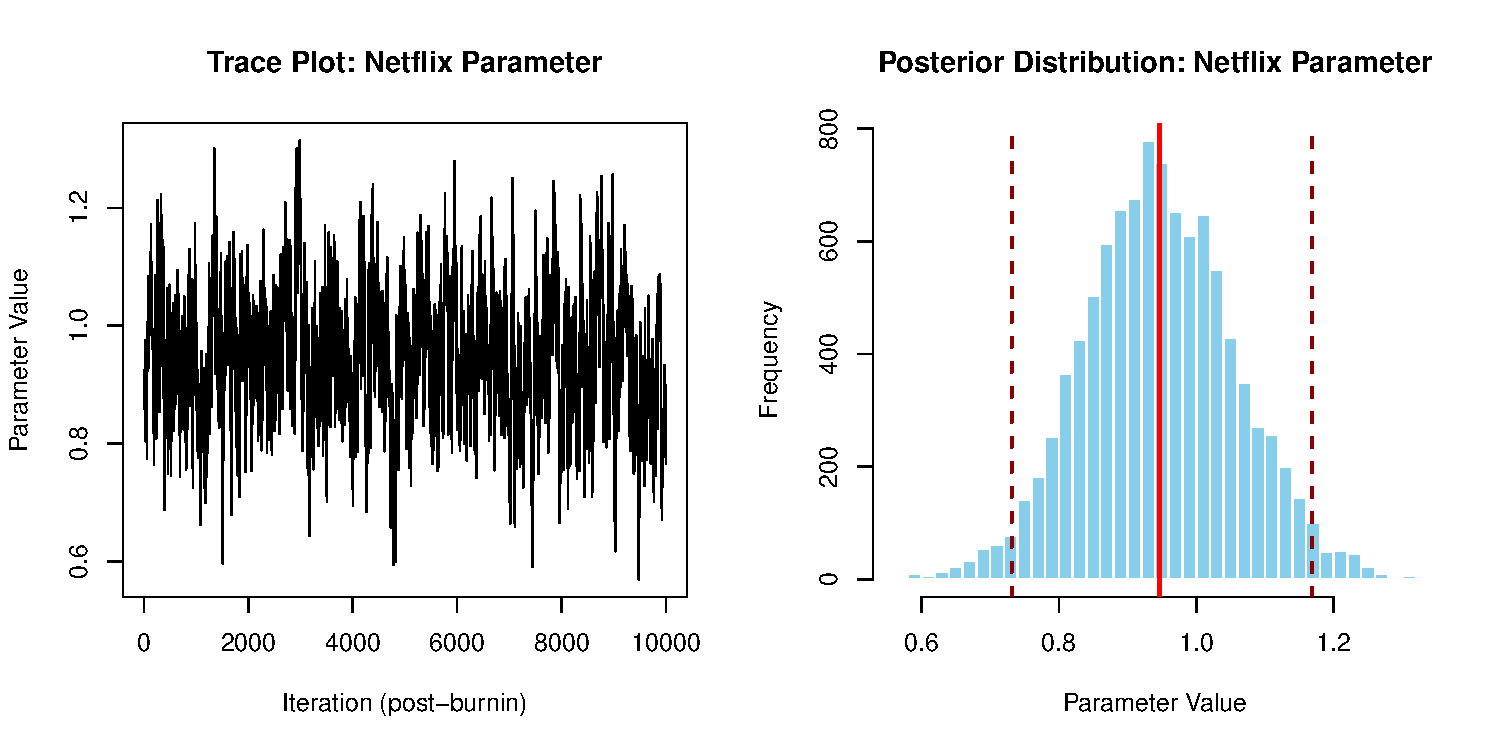
\includegraphics[keepaspectratio]{hw3_questions_files/figure-pdf/trace-hist-plots-1.pdf}}

}

\caption{Trace Plot and Posterior Distribution for Netflix Parameter}

\end{figure}%

\begin{Shaded}
\begin{Highlighting}[]
\FunctionTok{par}\NormalTok{(}\AttributeTok{mfrow =} \FunctionTok{c}\NormalTok{(}\DecValTok{1}\NormalTok{, }\DecValTok{1}\NormalTok{))}
\end{Highlighting}
\end{Shaded}

:::

The trace plot shows good mixing of the Markov chain, indicating
efficient exploration of the parameter space. The histogram shows the
posterior distribution is approximately normally distributed and
centered close to the true value of 1.0.

Let's calculate and report the posterior summaries: ::: \{.cell\}

\begin{Shaded}
\begin{Highlighting}[]
\CommentTok{\# Calculate posterior summary statistics}
\NormalTok{posterior\_means }\OtherTok{\textless{}{-}} \FunctionTok{colMeans}\NormalTok{(posterior\_samples)}
\NormalTok{posterior\_sds }\OtherTok{\textless{}{-}} \FunctionTok{apply}\NormalTok{(posterior\_samples, }\DecValTok{2}\NormalTok{, sd)}
\NormalTok{posterior\_ci }\OtherTok{\textless{}{-}} \FunctionTok{t}\NormalTok{(}\FunctionTok{apply}\NormalTok{(posterior\_samples, }\DecValTok{2}\NormalTok{, quantile, }\AttributeTok{probs =} \FunctionTok{c}\NormalTok{(}\FloatTok{0.025}\NormalTok{, }\FloatTok{0.975}\NormalTok{)))}
\end{Highlighting}
\end{Shaded}

:::

\begin{Shaded}
\begin{Highlighting}[]
\CommentTok{\# Create a summary table}
\NormalTok{bayes\_table }\OtherTok{\textless{}{-}} \FunctionTok{data.frame}\NormalTok{(}
  \AttributeTok{Parameter =} \FunctionTok{c}\NormalTok{(}\StringTok{"Netflix"}\NormalTok{, }\StringTok{"Prime"}\NormalTok{, }\StringTok{"Ads"}\NormalTok{, }\StringTok{"Price"}\NormalTok{),}
  \AttributeTok{Mean =} \FunctionTok{round}\NormalTok{(posterior\_means, }\DecValTok{3}\NormalTok{),}
  \AttributeTok{Std\_Dev =} \FunctionTok{round}\NormalTok{(posterior\_sds, }\DecValTok{3}\NormalTok{),}
  \AttributeTok{CI\_Lower =} \FunctionTok{round}\NormalTok{(posterior\_ci[, }\DecValTok{1}\NormalTok{], }\DecValTok{3}\NormalTok{),}
  \AttributeTok{CI\_Upper =} \FunctionTok{round}\NormalTok{(posterior\_ci[, }\DecValTok{2}\NormalTok{], }\DecValTok{3}\NormalTok{)}
\NormalTok{)}

\CommentTok{\# Display the Bayesian results}
\NormalTok{knitr}\SpecialCharTok{::}\FunctionTok{kable}\NormalTok{(bayes\_table, }
             \AttributeTok{caption =} \StringTok{"Bayesian Posterior Estimates"}\NormalTok{,}
             \AttributeTok{col.names =} \FunctionTok{c}\NormalTok{(}\StringTok{"Parameter"}\NormalTok{, }\StringTok{"Posterior Mean"}\NormalTok{, }\StringTok{"Posterior SD"}\NormalTok{, }
                           \StringTok{"95\% CI Lower"}\NormalTok{, }\StringTok{"95\% CI Upper"}\NormalTok{))}
\end{Highlighting}
\end{Shaded}

\begin{longtable}[]{@{}
  >{\raggedright\arraybackslash}p{(\linewidth - 10\tabcolsep) * \real{0.1111}}
  >{\raggedright\arraybackslash}p{(\linewidth - 10\tabcolsep) * \real{0.1389}}
  >{\raggedleft\arraybackslash}p{(\linewidth - 10\tabcolsep) * \real{0.2083}}
  >{\raggedleft\arraybackslash}p{(\linewidth - 10\tabcolsep) * \real{0.1806}}
  >{\raggedleft\arraybackslash}p{(\linewidth - 10\tabcolsep) * \real{0.1806}}
  >{\raggedleft\arraybackslash}p{(\linewidth - 10\tabcolsep) * \real{0.1806}}@{}}
\caption{Bayesian Posterior Estimates}\tabularnewline
\toprule\noalign{}
\begin{minipage}[b]{\linewidth}\raggedright
\end{minipage} & \begin{minipage}[b]{\linewidth}\raggedright
Parameter
\end{minipage} & \begin{minipage}[b]{\linewidth}\raggedleft
Posterior Mean
\end{minipage} & \begin{minipage}[b]{\linewidth}\raggedleft
Posterior SD
\end{minipage} & \begin{minipage}[b]{\linewidth}\raggedleft
95\% CI Lower
\end{minipage} & \begin{minipage}[b]{\linewidth}\raggedleft
95\% CI Upper
\end{minipage} \\
\midrule\noalign{}
\endfirsthead
\toprule\noalign{}
\begin{minipage}[b]{\linewidth}\raggedright
\end{minipage} & \begin{minipage}[b]{\linewidth}\raggedright
Parameter
\end{minipage} & \begin{minipage}[b]{\linewidth}\raggedleft
Posterior Mean
\end{minipage} & \begin{minipage}[b]{\linewidth}\raggedleft
Posterior SD
\end{minipage} & \begin{minipage}[b]{\linewidth}\raggedleft
95\% CI Lower
\end{minipage} & \begin{minipage}[b]{\linewidth}\raggedleft
95\% CI Upper
\end{minipage} \\
\midrule\noalign{}
\endhead
\bottomrule\noalign{}
\endlastfoot
Netflix & Netflix & 0.947 & 0.110 & 0.732 & 1.169 \\
Prime & Prime & 0.503 & 0.109 & 0.289 & 0.732 \\
Ads & Ads & -0.736 & 0.092 & -0.913 & -0.549 \\
Price & Price & -0.100 & 0.006 & -0.113 & -0.088 \\
\end{longtable}

\begin{Shaded}
\begin{Highlighting}[]
\CommentTok{\# Compare with MLE results}
\NormalTok{comparison\_table }\OtherTok{\textless{}{-}} \FunctionTok{data.frame}\NormalTok{(}
  \AttributeTok{Parameter =} \FunctionTok{c}\NormalTok{(}\StringTok{"Netflix"}\NormalTok{, }\StringTok{"Prime"}\NormalTok{, }\StringTok{"Ads"}\NormalTok{, }\StringTok{"Price"}\NormalTok{),}
  \AttributeTok{MLE =} \FunctionTok{round}\NormalTok{(beta\_mle, }\DecValTok{3}\NormalTok{),}
  \AttributeTok{MLE\_CI\_Lower =} \FunctionTok{round}\NormalTok{(ci\_lower, }\DecValTok{3}\NormalTok{),}
  \AttributeTok{MLE\_CI\_Upper =} \FunctionTok{round}\NormalTok{(ci\_upper, }\DecValTok{3}\NormalTok{),}
  \AttributeTok{Bayes\_Mean =} \FunctionTok{round}\NormalTok{(posterior\_means, }\DecValTok{3}\NormalTok{),}
  \AttributeTok{Bayes\_CI\_Lower =} \FunctionTok{round}\NormalTok{(posterior\_ci[, }\DecValTok{1}\NormalTok{], }\DecValTok{3}\NormalTok{),}
  \AttributeTok{Bayes\_CI\_Upper =} \FunctionTok{round}\NormalTok{(posterior\_ci[, }\DecValTok{2}\NormalTok{], }\DecValTok{3}\NormalTok{)}
\NormalTok{)}

\CommentTok{\# Display the comparison}
\NormalTok{knitr}\SpecialCharTok{::}\FunctionTok{kable}\NormalTok{(comparison\_table, }
             \AttributeTok{caption =} \StringTok{"Comparison: MLE vs Bayesian Estimates"}\NormalTok{,}
             \AttributeTok{col.names =} \FunctionTok{c}\NormalTok{(}\StringTok{"Parameter"}\NormalTok{, }\StringTok{"MLE Estimate"}\NormalTok{, }\StringTok{"MLE 95\% CI Lower"}\NormalTok{, }\StringTok{"MLE 95\% CI Upper"}\NormalTok{,}
                           \StringTok{"Bayes Mean"}\NormalTok{, }\StringTok{"Bayes 95\% CI Lower"}\NormalTok{, }\StringTok{"Bayes 95\% CI Upper"}\NormalTok{))}
\end{Highlighting}
\end{Shaded}

\begin{longtable}[]{@{}
  >{\raggedright\arraybackslash}p{(\linewidth - 14\tabcolsep) * \real{0.0702}}
  >{\raggedright\arraybackslash}p{(\linewidth - 14\tabcolsep) * \real{0.0877}}
  >{\raggedleft\arraybackslash}p{(\linewidth - 14\tabcolsep) * \real{0.1140}}
  >{\raggedleft\arraybackslash}p{(\linewidth - 14\tabcolsep) * \real{0.1491}}
  >{\raggedleft\arraybackslash}p{(\linewidth - 14\tabcolsep) * \real{0.1491}}
  >{\raggedleft\arraybackslash}p{(\linewidth - 14\tabcolsep) * \real{0.0965}}
  >{\raggedleft\arraybackslash}p{(\linewidth - 14\tabcolsep) * \real{0.1667}}
  >{\raggedleft\arraybackslash}p{(\linewidth - 14\tabcolsep) * \real{0.1667}}@{}}
\caption{Comparison: MLE vs Bayesian Estimates}\tabularnewline
\toprule\noalign{}
\begin{minipage}[b]{\linewidth}\raggedright
\end{minipage} & \begin{minipage}[b]{\linewidth}\raggedright
Parameter
\end{minipage} & \begin{minipage}[b]{\linewidth}\raggedleft
MLE Estimate
\end{minipage} & \begin{minipage}[b]{\linewidth}\raggedleft
MLE 95\% CI Lower
\end{minipage} & \begin{minipage}[b]{\linewidth}\raggedleft
MLE 95\% CI Upper
\end{minipage} & \begin{minipage}[b]{\linewidth}\raggedleft
Bayes Mean
\end{minipage} & \begin{minipage}[b]{\linewidth}\raggedleft
Bayes 95\% CI Lower
\end{minipage} & \begin{minipage}[b]{\linewidth}\raggedleft
Bayes 95\% CI Upper
\end{minipage} \\
\midrule\noalign{}
\endfirsthead
\toprule\noalign{}
\begin{minipage}[b]{\linewidth}\raggedright
\end{minipage} & \begin{minipage}[b]{\linewidth}\raggedright
Parameter
\end{minipage} & \begin{minipage}[b]{\linewidth}\raggedleft
MLE Estimate
\end{minipage} & \begin{minipage}[b]{\linewidth}\raggedleft
MLE 95\% CI Lower
\end{minipage} & \begin{minipage}[b]{\linewidth}\raggedleft
MLE 95\% CI Upper
\end{minipage} & \begin{minipage}[b]{\linewidth}\raggedleft
Bayes Mean
\end{minipage} & \begin{minipage}[b]{\linewidth}\raggedleft
Bayes 95\% CI Lower
\end{minipage} & \begin{minipage}[b]{\linewidth}\raggedleft
Bayes 95\% CI Upper
\end{minipage} \\
\midrule\noalign{}
\endhead
\bottomrule\noalign{}
\endlastfoot
Netflix & Netflix & 0.941 & 0.724 & 1.159 & 0.947 & 0.732 & 1.169 \\
Prime & Prime & 0.502 & 0.284 & 0.719 & 0.503 & 0.289 & 0.732 \\
Ads & Ads & -0.732 & -0.904 & -0.560 & -0.736 & -0.913 & -0.549 \\
Price & Price & -0.099 & -0.112 & -0.087 & -0.100 & -0.113 & -0.088 \\
\end{longtable}

The Bayesian estimates are very similar to the MLE estimates, which is
expected given the large sample size and the relatively uninformative
priors. Both methods recover the true parameter values quite well, with
the posteriors showing slightly wider credible intervals compared to the
confidence intervals from MLE.

\subsection{6. Discussion}\label{discussion}

The parameter estimates from both the MLE and Bayesian approaches align
closely with the true values used in the simulation
(\(\beta_\text{netflix} = 1.0\), \(\beta_\text{prime} = 0.5\),
\(\beta_\tex{ads} = -.08\), \(\beta_\text{price} = -0.1\)). This
confirms that our estimation methods are working correctly.

The interpretation of these parameters provides meaningful insights into
consumer preferences:

Brand preferences: The positive and significant coefficients for Netflix
(approximately 1.0) and Prime (approximately 0.5) indicate that
consumers prefer these brands over Hulu (the reference level). Further,
the fact that βₙₑₜfₗᵢₓ \textgreater{} βₚᵣᵢₘₑ means that, all else equal,
consumers have a stronger preference for Netflix than for Amazon Prime.
In particular, the odds of choosing Netflix over Hulu (if all other
attributes are identical) is approximately e¹·⁰ = 2.7, while the odds of
choosing Prime over Hulu is approximately e⁰·⁵ = 1.6.

Ad preference: The negative coefficient for ads (approximately -0.8)
indicates that, as expected, consumers dislike advertising in their
streaming services. The presence of ads reduces utility and thus
decreases the probability of choosing a service with ads, all else
equal.

Price sensitivity: The negative coefficient for price (approximately
-0.1) reflects that consumers are price-sensitive. As the price
increases, the utility decreases, and consequently, the probability of
choosing that service decreases. This makes economic sense as consumers
typically prefer lower prices.

To extend this model to a multi-level (hierarchical) framework, several
key changes would be required:

Parameter heterogeneity: Instead of assuming all respondents have the
same preferences (βs), we would model individual-level parameters that
vary across respondents according to a distribution: β\_i
\textasciitilde{} MVN(μ\_β, Σ\_β)

where β\_i represents the vector of preference parameters for respondent
i, μ\_β is the vector of population means, and Σ\_β is the covariance
matrix capturing heterogeneity across respondents.

Estimation approach: The Bayesian MCMC approach would need to be
modified to sample both the individual-level parameters (β\_i) and the
population-level hyperparameters (μ\_β and Σ\_β). This typically
involves using a Gibbs sampler with Metropolis-Hastings steps.

Data structure: The data preparation would remain similar, but we would
need to keep track of respondent identities more carefully to model the
within-respondent correlation in choices.

Computational complexity: The model would become significantly more
complex, with hundreds of parameters to estimate (4 parameters per
respondent × 100 respondents, plus population parameters), requiring
more efficient MCMC algorithms and potentially more computational
resources.

Prior specifications: We would need to specify priors not only for the
mean parameters but also for the covariance matrix, typically using an
Inverse-Wishart distribution.

A hierarchical model would provide richer insights by capturing
preference heterogeneity across respondents, allowing for personalized
predictions and targeted marketing strategies. However, this comes at
the cost of increased model complexity and computational demands.




\end{document}
